\documentclass[a4paper, 12pt, leqno]{report}

\usepackage[T1]{fontenc}
\usepackage[utf8x]{inputenc}
\usepackage[greek,french, \frenchb]{babel}
\usepackage[babel=true]{csquotes}
\usepackage[top=1.5cm, bottom=2.0cm, left=2.0cm, right=2.0cm]{geometry}
\usepackage{fancyhdr}
\usepackage{graphicx}
\usepackage{amsmath}
\usepackage{soul}
\usepackage{amssymb}
\pagestyle{plain}
\usepackage{amsfonts}
\usepackage{amssymb}
\usepackage{amsthm}
\usepackage{graphicx}
\usepackage{color}
\usepackage{enumerate}
\usepackage{array}
\theoremstyle{plain}
\usepackage{blkarray}
\usepackage{listings}
\usepackage{algorithmicx}
\usepackage{algpseudocode}
\usepackage{algorithm}
\usepackage{lscape}
\usepackage{pdflscape}
\usepackage{eurosym}

\usepackage{caption}
\DeclareCaptionFont{white}{\color{white}}
\DeclareCaptionFormat{listing}{\colorbox{black}{\parbox{\textwidth}{#1#2#3}}}
\captionsetup[lstlisting]{format=listing,labelfont=white,textfont=white}

\frenchbsetup{StandardLists=true}
\renewcommand{\labelitemi}{\textbullet}

\newcommand{\bigO}[1]{\ensuremath{\mathop{}\mathopen{}O\mathopen{}\left(#1\right)}}
\newcommand{\smallO}[1]{\ensuremath{\mathop{}\mathopen{}o\mathopen{}\left(#1\right)}}

\begin{document}

\begin{titlepage}

\newcommand{\HRule}{\rule{\linewidth}{0.5mm}} % Defines a new command for the horizontal lines, change thickness here

\center % Center everything on the page
 
%----------------------------------------------------------------------------------------
%	HEADING SECTIONS
%----------------------------------------------------------------------------------------

\textsc{\LARGE Université de Technologie de Compiègne}\\[1.5cm] % Name of your university/college
\textsc{\Large GE37}\\[0.5cm] % Major heading such as course name
\textsc{\large Management de projets}\\[0.5cm] % Minor heading such as course title

%----------------------------------------------------------------------------------------
%	TITLE SECTION
%----------------------------------------------------------------------------------------

\HRule \\[0.4cm]
{ \huge \bfseries Rapport sur le projet de conception de Mini-drône}\\[0.4cm] % Title of your document
\HRule \\[1.5cm]
 
%----------------------------------------------------------------------------------------
%	AUTHOR SECTION
%----------------------------------------------------------------------------------------

\begin{minipage}{0.4\textwidth}
\begin{flushleft} \large
\emph{Auteurs :}\\
Romain \textsc{BUTTEAUD} % Your name
Damien \textsc{MARIÉ} 
Wangfan \textsc{LI} 
Minh \textsc{LE} 
Antoine \textsc{POUILLAUDE} 
\end{flushleft}
\end{minipage}
~
\begin{minipage}{0.4\textwidth}
\begin{flushright} \large
\emph{Chef de projet :} \\
Damien \textsc{MAIRIÉ} \\% Supervisor's Name
\emph{Porteur du projet :} \\
Jérôme \textsc{DEMIRAS} % Supervisor's Name
\end{flushright}
\end{minipage}\\[4cm]

% If you don't want a supervisor, uncomment the two lines below and remove the section above
%\Large \emph{Author:}\\
%John \textsc{Smith}\\[3cm] % Your name

%----------------------------------------------------------------------------------------
%	DATE SECTION
%----------------------------------------------------------------------------------------

{\large \today}\\[3cm] % Date, change the \today to a set date if you want to be precise

%----------------------------------------------------------------------------------------
%	LOGO SECTION
%----------------------------------------------------------------------------------------

\includegraphics[scale=0.5]{Files/Logo_UTC}\\[1cm] % Include a department/university logo - this will require the graphicx package
 
%----------------------------------------------------------------------------------------

\vfill % Fill the rest of the page with whitespace

\end{titlepage}
    \tableofcontents
    \listoffigures
\newpage
\section*{Introduction}
        Ce document ne se veut en aucun cas être un dossier de définition du projet. Il s'agit plus d'un résumé des différents fichier que nous avons produit jusqu'ici dans le cadre de notre étude de cas flux. Il regroupe les différents outils de définition du projet à savoir : une note de clarification, un diagramme PDP, tout les outils de découpage et de structuration du projet, un budget de référence et une analyse des risques. Ces documents seront commentés de manière concise faute de temps.
        \chapter{Note de clarification}
        \section{Contexte}  
        Le laboratoire informatique de l'UTC souhaite s'équiper d'une flotte de drône pour mettre en application leurs recherches sur le compartement intelligent d'un groupe de drônes dans des applications civiles. Pour cela, une équipe étudiante de l'association Fablab'UTC (ayant pour but de promouvoir la création d'un atelier étudiant à l'UTC) qui a déjà collaboré avec le laboratoire Heudiasyc, va concevoir le drône.
        \section{Données d'entrée}
        \begin{itemize}
        \item Expérience de collaboration Fablab'UTC-Heudiasyc
        \item Expérience des membres de Fablab'UTC dans le domaine des drônes.
        \item Machines de prototypage et matèriel de Fablab'UTC et Heudiasyc.
        \item Expérience de l'équipe Heudiasyc sur la conception de nombreux drônes.
        \item Cahier des charges.
        \end{itemize}
         
        \section{Objet}
        Le projet consiste d'abord à mettre au clair les besoins exacts et les contraintes techniques. Puis suivra la conception d'un mini-drône respectant ce cahier des charges.
        \section{Produits du projet}
        \begin{itemize}
        \item Spécifications techniques du drône et un dossier de conception.
        \item Un prototype fonctionel.
        \end{itemize}
        
        \section{Objectifs}
        \begin{itemize}
        \item Conception totale terminée avant le 1 janvier 2014.
        \item Coût inférieur à 1000 \euro par drône.
        \item Apprentissage de la conception de drône à des étudiants.
        \end{itemize}

        \section{Acteurs}
        \begin{description}
        \item[Maîtrise d'ouvrage :] Heudiasyc
        \item[Maîtrise d'oeuvre :] Fablab'UTC
        \item[Partenaires :] Université de Technologie de Compiègne
        \item[Fournisseurs :] Fablab'UTC, UTC et Heudiasyc
        \end{description}
        \section{Conséquences attendues}
        Permettre au laboratoire Heudiasyc d'avancer sur ses recherches et les applications.
        Apprendre à des étudiants la conception de drône.
        Communication positive pour Fablab'UTC et Heudiasyc.
        
        \section{Contraintes}
        Le code source d ela partie commande du Mini-Drône est protégé.
        On doit utiliser l'électronique de commande qu'Heudiasyc utilise sur ses propres drônes.
        La structure dudrône devra être imprimmable par une imprimante 3D.

        \chapter{Structuration du projet}
        \begin{landscape}
        \section{PDP}
           \begin{figure}[H]
           \begin{center}
           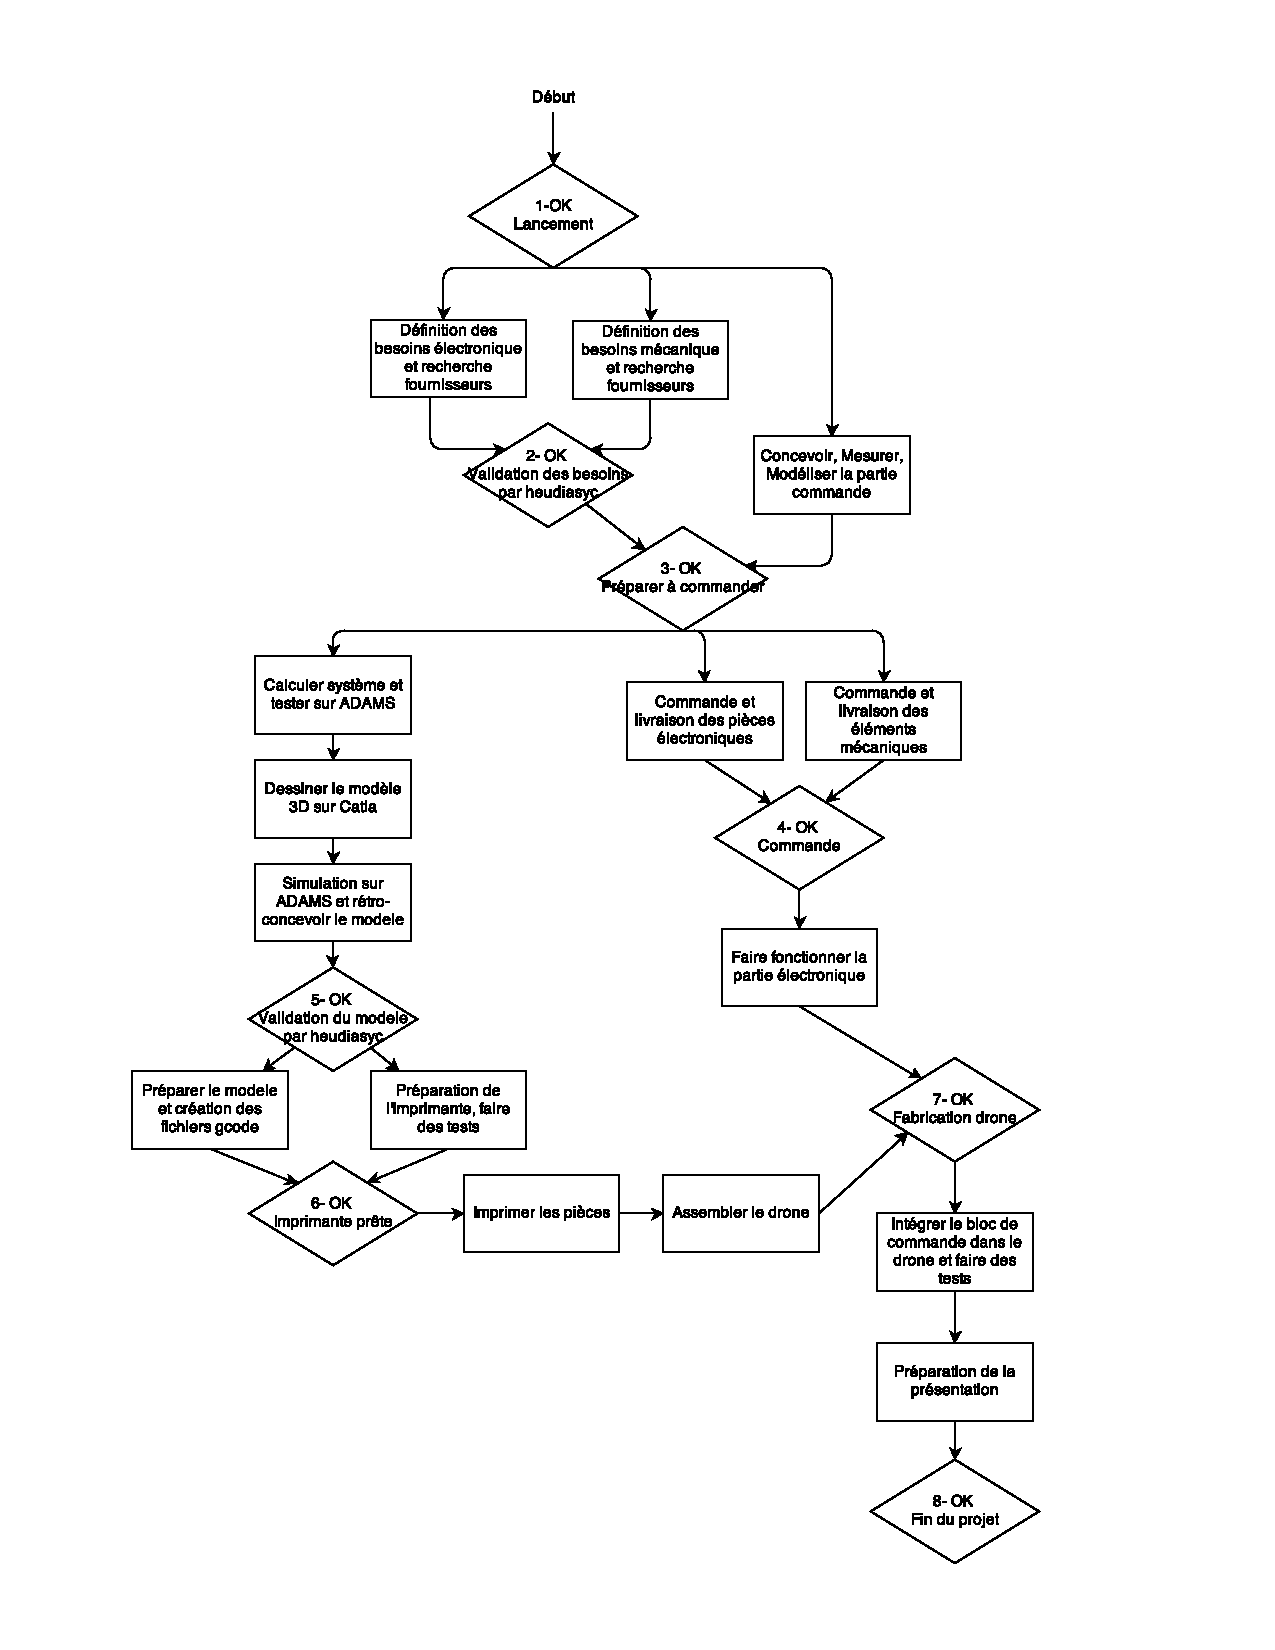
\includegraphics[height=255mm, width=140mm, angle=90]{Files/PDPProject.pdf}
           \end{center}
           \caption{Processus de Développement du Projet}
           \label{Processus de Développement du Projet}
           \end{figure}

        \section{Product Breakdown Structure}
        \begin{figure}[H]
           \begin{center}
           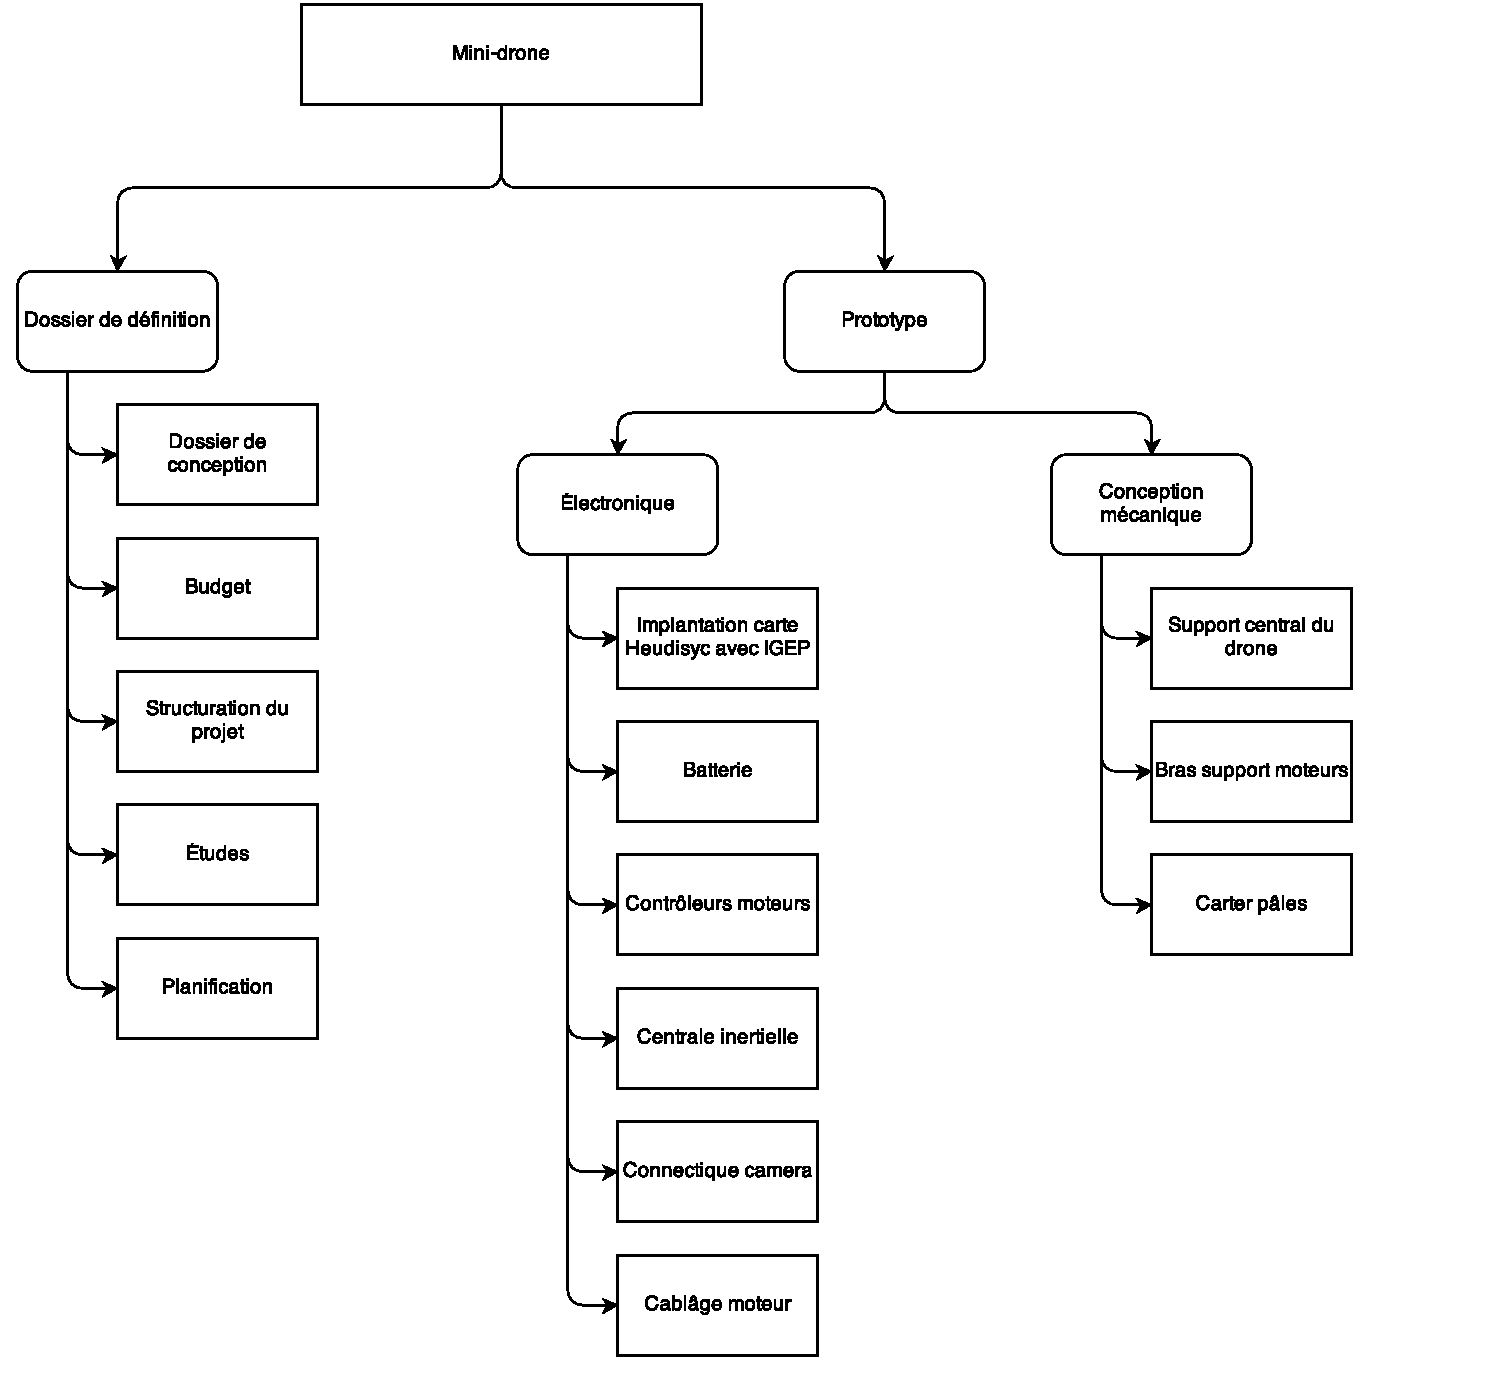
\includegraphics[height=200mm, width=140mm, angle=90]{Files/PBS.pdf}
           \end{center}
           \caption{Product Breakdown Structure Diagram}
           \label{Product Breakdown Structure Diagram}
           \end{figure}
           
        \section{Working Breakdown Structure}
        \begin{figure}[H]
           \begin{center}
           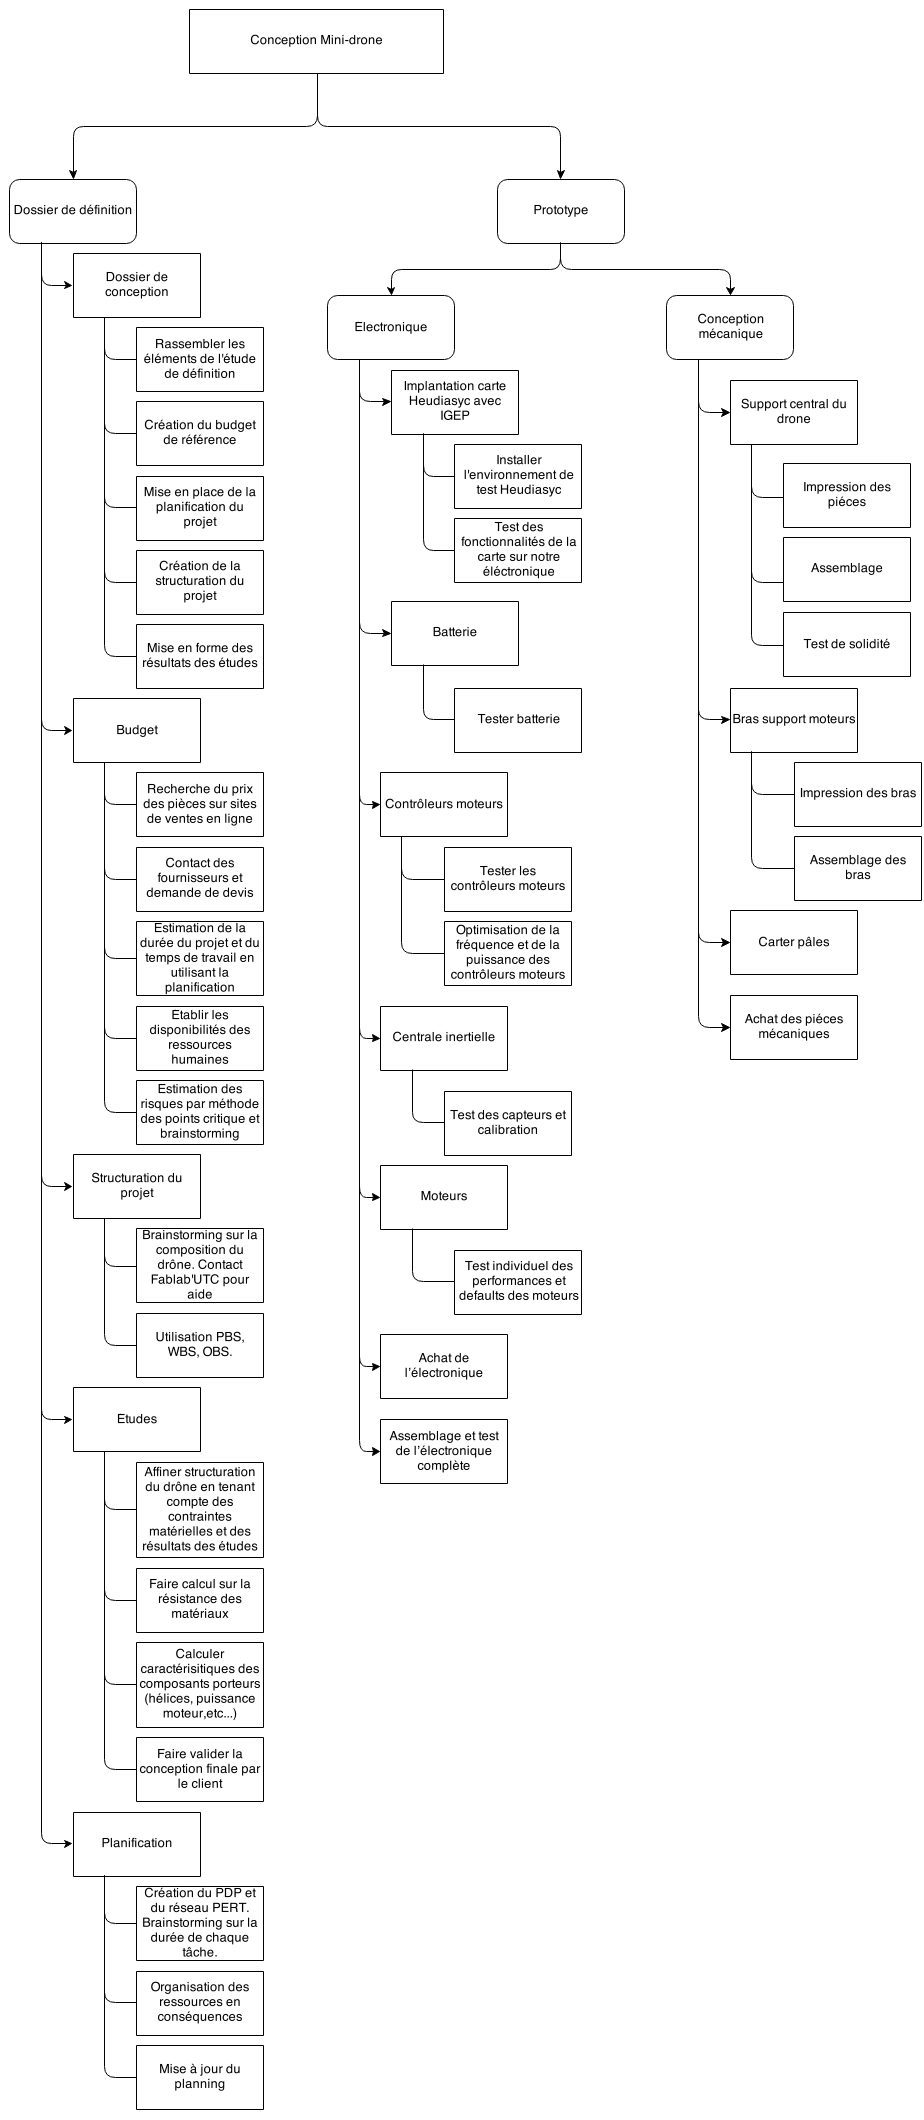
\includegraphics[height=255mm, width=140mm, angle=90]{Files/WBS_review_v3.png}
           \end{center}
           \caption{Working Breakdown Structure Diagram}
           \label{Working Breakdown Structure Diagram}
           \end{figure}
           
        \section{Organisational Breakdown Structure}
        \begin{figure}[H]
           \begin{center}
           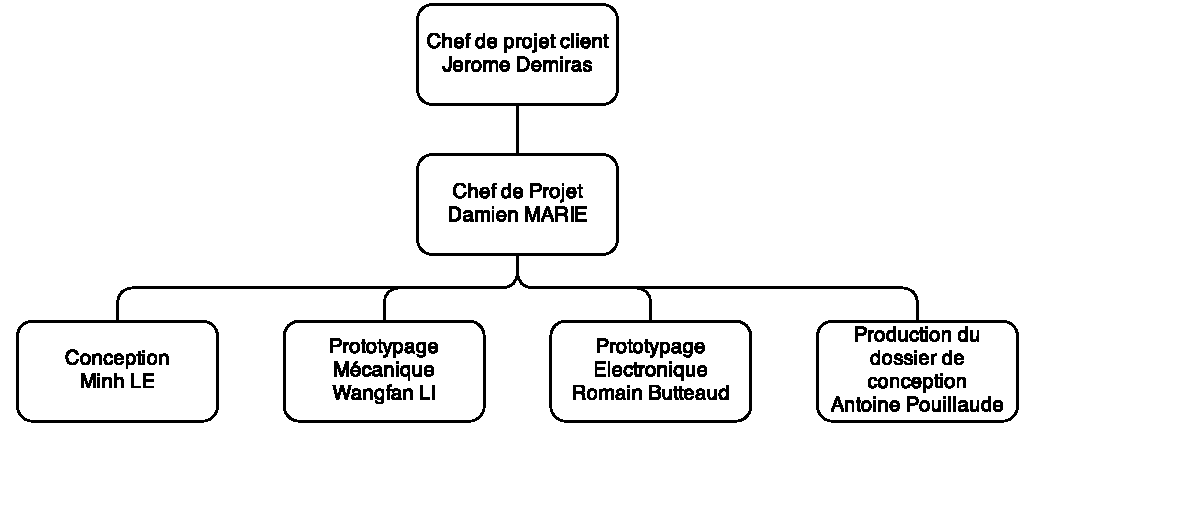
\includegraphics[scale=1.5]{Files/OBSProject_review_v2.pdf}
           \end{center}
           \caption{Organisational Breakdown Structure Diagram}
           \label{Organisational Breakdown Structure Diagram}
           \end{figure}
           \section{PERT}
           \begin{figure}[H]
           \begin{center}
           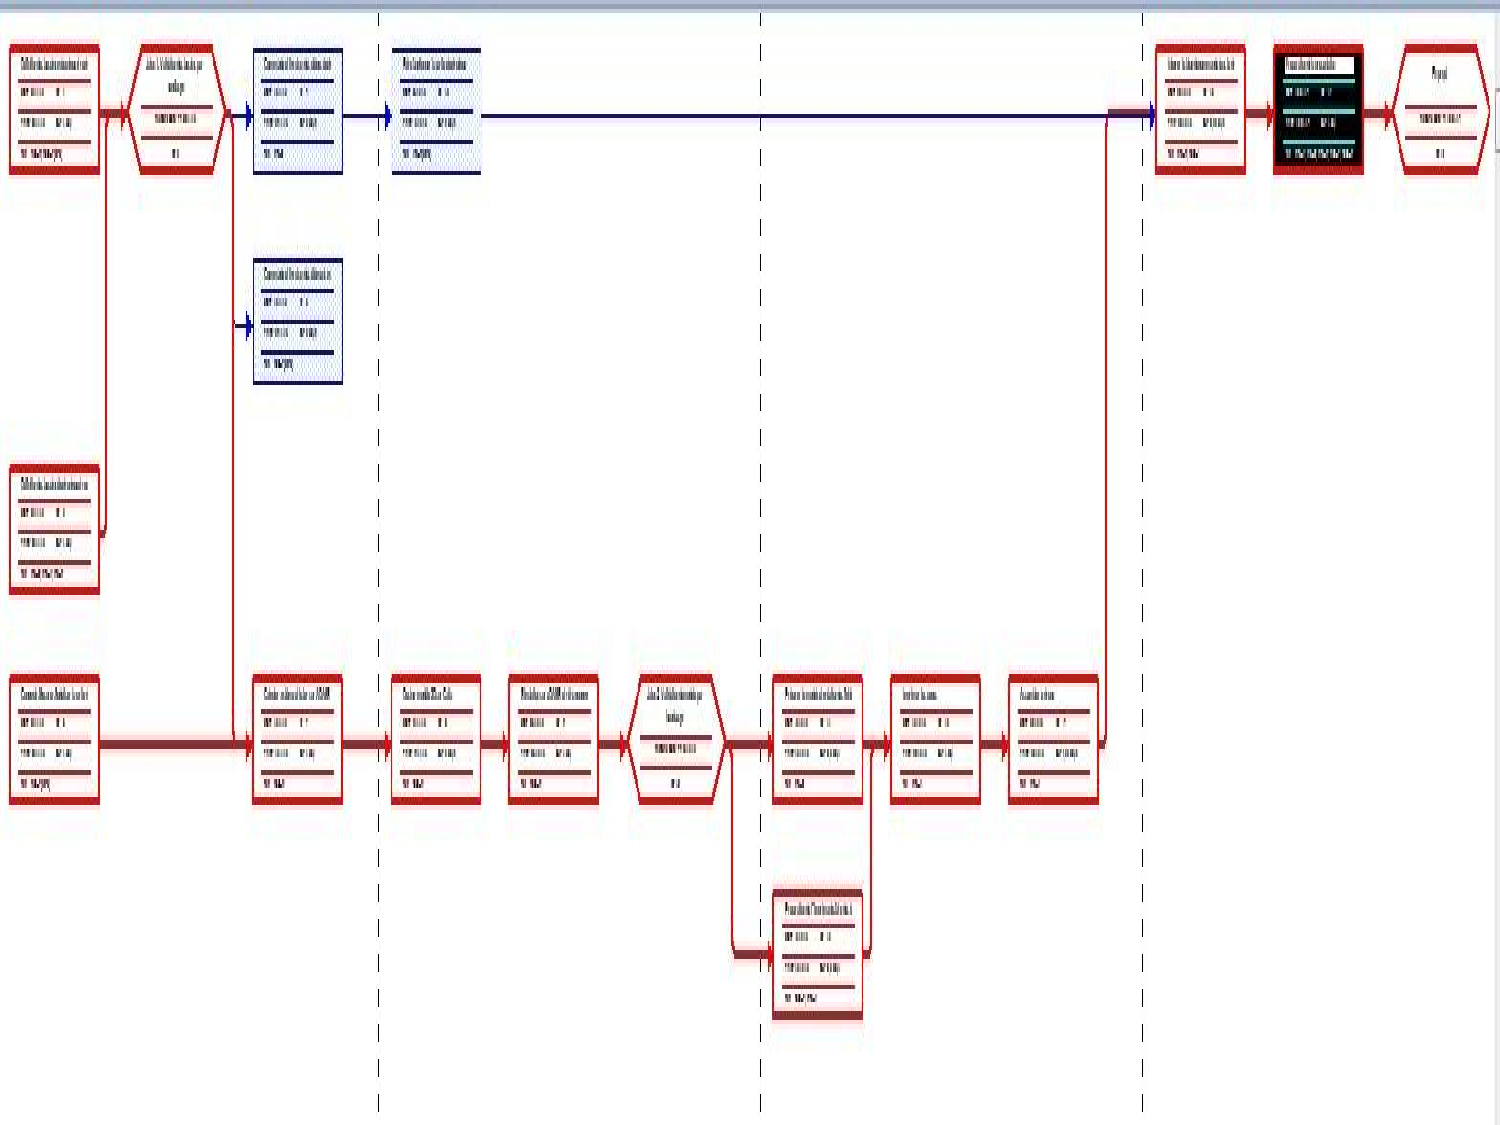
\includegraphics[scale=0.75]{Files/Pert.pdf}
           \end{center}
           \caption{Diagramme Pert. Pour avoir une version plus lisible se réferrer au fichier ".mpp"}
           \label{Diagramme Pert.}
           \end{figure}
           \section{Diagramme de Gantt}
           \begin{figure}[H]
           \begin{center}
           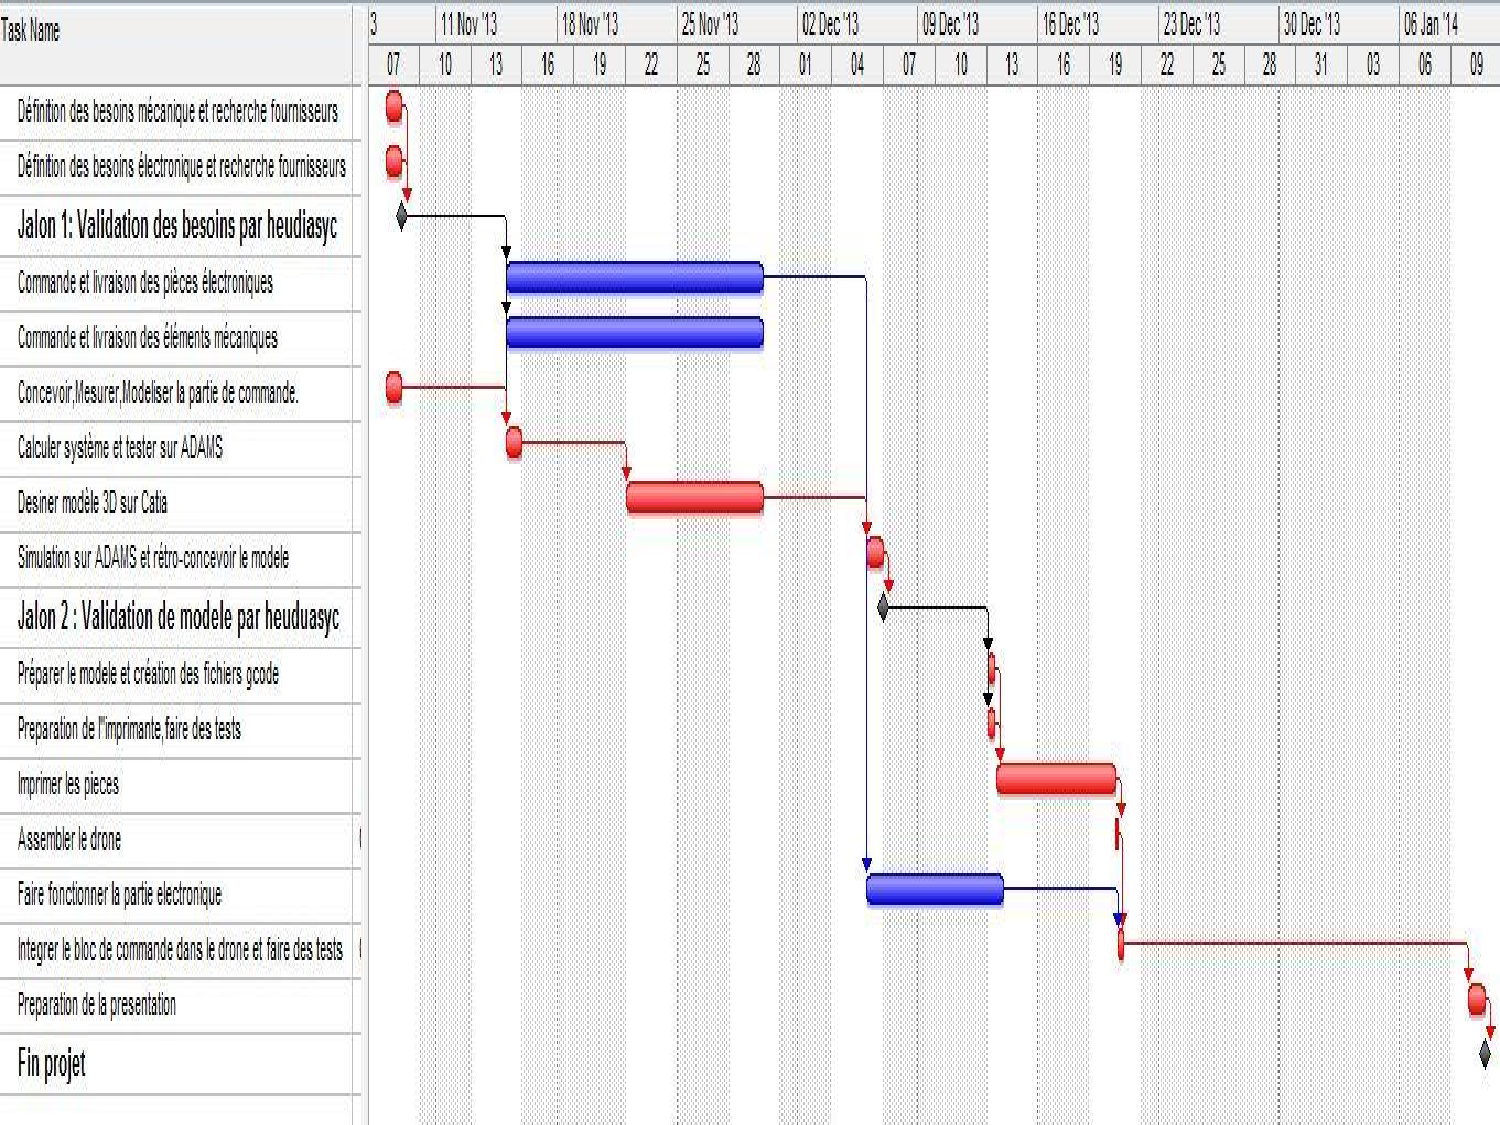
\includegraphics[scale=0.75]{Files/Gantt.pdf}
           \end{center}
           \caption{Diagramme de Gantt. Pour avoir une version plus lisible se réferrer au fichier ".mpp"}
           \label{Diagramme Gantt}
           \end{figure}
           \end{landscape}
           \chapter{Études et analyses}
           \section{Budget de référence}
           \begin{figure}[H]
           \begin{center}
           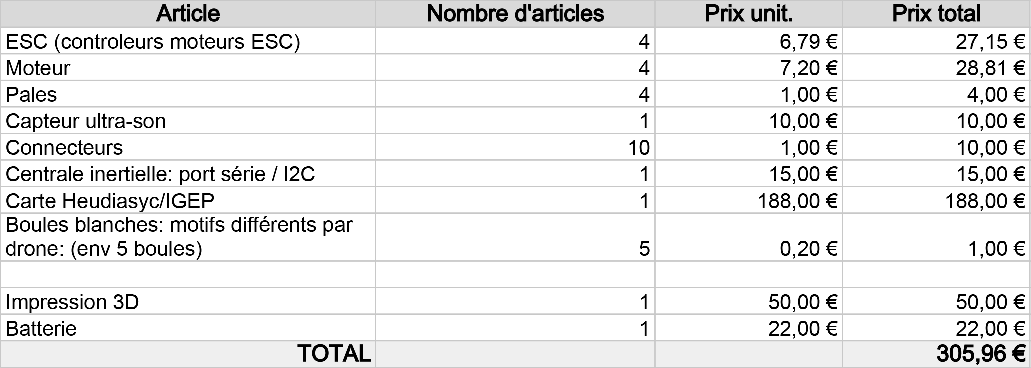
\includegraphics[scale=0.75]{Files/Budget_Achat_Composants.pdf}
           \end{center}
           \caption{Budget de référence}
           \label{Budget de référence}
           \end{figure}
           \section{Analyse des risques}
            \subsection{Points critiques}
            Compétences : 
            \begin{itemize}
            \item Risque de manque de compétence pour gérer les parties mécaniques
            \item Risque de manque de compétence pour gérer la partie informatique.
            \item Risque de mauvaise compréhension des objectifs du projet
            \end{itemize}
            Fournisseur :
            \begin{itemize}
            \item Risque de ne pas bien communiquer avec les fournisseurs.
            \item Risque de ne pas obtenir les matériaux
            \item Risque de recevoir des matériaux de qualité moindre.
            \end{itemize}
            Technologie éprouvée :
            \begin{itemize}
            \item Risque d'une mauvaise répartition du travail.
            \item Risque de manque de connaissance dû aux changement de certains paramètres
            \end{itemize}
            Parmis ces points critiques nous en avons sélectionné trois, un dans chaque catégorie. Ces points critiques sont détaillés ci-après.
              \subsubsection{Risque de mauvaise compréhension des objectifs du projet}
              \begin{description}
              \item[Cause :] Le projet est complexe et les contraintes imprécises
              \item[Effet :] Le produit ne peut pas fonctionner correctement ou ne répond pas aux attentes fixées.
              \item[Plan d'action :] ARE : Encadrement renforcé du porteur et/ou du chef de projet.
              \end{description}
              \subsubsection{Risque de recevoir des matériaux de qualité moindre}
              \begin{description}
              \item[Cause :] Les fournisseurs n'ont pas été choisis de manière réfléchie.
              \item[Effet :] Le produit présente une structure fragile.
              \item[Plan d'action :] ARC : Renforcer la communication avec les fournisseurs afin de s'assurer de la qualité de matériaux.
              \end{description}
              \subsubsection{Risque d'une mauvaise répartition du travail}
              \begin{description}
              \item[Cause :] Mauvaise appréciation des durées des tâches et du temps de travail.
              \item[Effet :] Ressources mal-exploitées et dépassement des délais.
              \item[Plan d'action :] ADA : Vérification de la charge de travail de chacun par le chef de projet. Effort d'estimation du temps des tâches.
              \end{description}
              
              Nous rappelons la signification des abbréviations utilisées ci-dessus :
              \begin{description}
              \item[ARC :] Action en Réduction des Causes
              \item[ARE :] Action en Réduction des Effets
              \item[ADA :] Action pour Détecter l'Apparition.
              \end{description}
              \begin{itemize}
              \item[G :] Gravité (1,3,6,9)
              \item[A :] Probabilité d'apparition (1,3,6,9)
              \item[D :] Probabulité de non-détection (1,3,6,9)
              \end{itemize}
              Criticité = $G*A*D$
    \begin{figure}[H]
           \begin{center}
           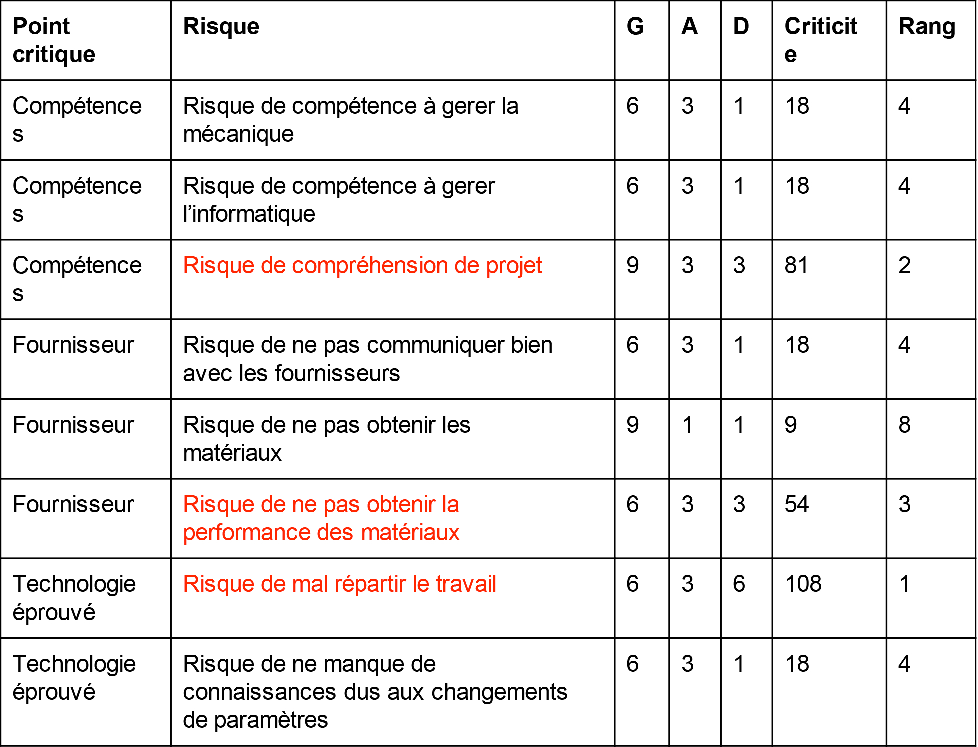
\includegraphics[scale=0.75]{Files/Analyse_des_risques.pdf}
           \end{center}
           \caption{Tableau récapitulatif du Brainstorming effectué}
           \label{Tableau récapitulatif du Brainstorming effectué}
           \end{figure}

     
                     
              
   
                
\end{document}
